\documentclass{article} % For LaTeX2e
\usepackage[backend=bibtex, sorting=none]{biblatex}
\addbibresource{bibliography.bib}
\usepackage{nips15submit_e,times}
\usepackage{hyperref}
\usepackage{url}
\usepackage{amsmath}
\usepackage{tipa}
\usepackage{multicol}
\usepackage{multirow}
\usepackage{array}
\usepackage{graphicx}
\usepackage{bm}
\usepackage{mathtools,xparse}
\graphicspath{ {figures/} }
\newcolumntype{P}[1]{>{\centering\arraybackslash}p{#1}}
\usepackage[linesnumberedhidden,ruled,noend]{algorithm2e}

\makeatletter
\def\BState{\State\hskip-\ALG@thistlm}
\makeatother
%\documentstyle[nips14submit_09,times,art10]{article} % For LaTeX 2.09

\title{COMPGZ05: Multimedia Systems - Coursework}

\author{
Sergiu Tripon\\
Department of Computer Science\\
University College London\\
Gower Street, London, WC1E\\
\texttt{sergiu.tripon.15@ucl.ac.uk}\\
}

% The \author macro works with any number of authors. There are two commands
% used to separate the names and addresses of multiple authors: \And and \AND.
%
% Using \And between authors leaves it to \LaTeX{} to determine where to break
% the lines. Using \AND forces a linebreak at that point. So, if \LaTeX{}
% puts 3 of 4 authors names on the first line, and the last on the second
% line, try using \AND instead of \And before the third author name.

\newcommand{\fix}{\marginpar{FIX}}
\newcommand{\new}{\marginpar{NEW}}

\nipsfinalcopy % Uncomment for camera-ready version

\begin{document}

\maketitle

\section{Interpolation - Algorithm Description}

The gap is calculated. If the gap is shorter/equal than/to three packets, we calculate the DCT of the packets before and after the gap. If the gap is exactly one packet, we calculate the missing sequence number, and while the missing sequence number is less than the current sequence number, we create a new set of coefficients and fill it with the average of the DCT coefficients. We calculate the IDCT of the new set of coefficients. We fill the gap with the IDCT of the interpolated DCT coefficients. We increment the missing sequence number. If the gap is exactly two or three packets long, we calculate the missing sequence number, and while the missing sequence number is less than the current sequence number, we calculate a weighted average for each missing packet. We create a new set of coefficients and fill it with the sum of the products of the weighted averages and DCT coefficients. We calculate the IDCT of the new set of coefficients. We fill the gap with the IDCT of the new interpolated DCT coefficients. We increment the missing sequence number. If the gap is longer than 3 packets, we fill the gap with silence. The figure below presents a comparison between the silence (top) and the completed interpolate (bottom) repair strategies.

\begin{figure}[!htbp]
\centering
\fbox{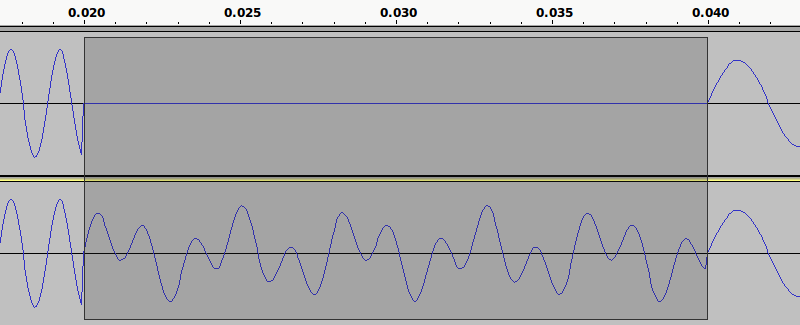
\includegraphics[width=13.7cm]{interpolation}}
\end{figure}

\section{Smoothing - Algorithm Description}

The gap and steps are calculated. If there is one sample, the step is 0.5 and if there are two samples, the steps are 0.3333 and 0.6667. We fill the gap with the last half of the previous packet, except the penultimate and last sample.We calculate the penultimate and last sample of the previous packet. We fill the gap with the penultimate sample followed by the last sample of the previous packet. We calculate the first and second sample of the current packet. We fill the gap with the first sample followed by the second sample of the current packet.We fill the gap with the first half of the current packet, except the first and second sample. The figure below presents a comparison between the repeat both repair strategy with smoothing disabled (top) and enabled (bottom).

\begin{figure}[!htbp]
\centering
\fbox{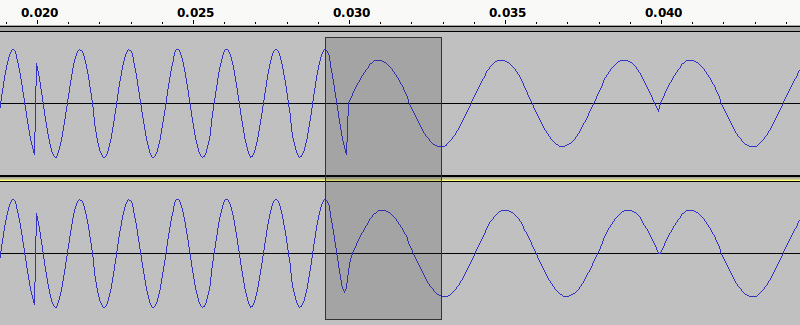
\includegraphics[width=13.7cm]{smoothing}}
\end{figure}

\section{Repair Efficiency - Explanation}

I believe that interpolate repair strategy does the best job at repairing loss. Using interpolation, the created audio is a mix of the audio before and after the gap. In contrast, repeat both tries to achieve this, but tackles the problem in a basic way. It simply fills the gap with the last half of the previous packet and the first half of the current packet. This means the resulting repaired packet will always be split in half. Furthermore, in comparison to interpolation, using any of the other repair strategy means that the edges of the repaired packet will not match the edges of the other packets. This can be fixed using smoothing, but requires further work. Smoothing is not required in interpolation.

\end{document}